%!TEX root = ../hbrs-poster.tex

\block{Results}
{
    \begin{center}
        \begin{minipage}{0.48\linewidth}
            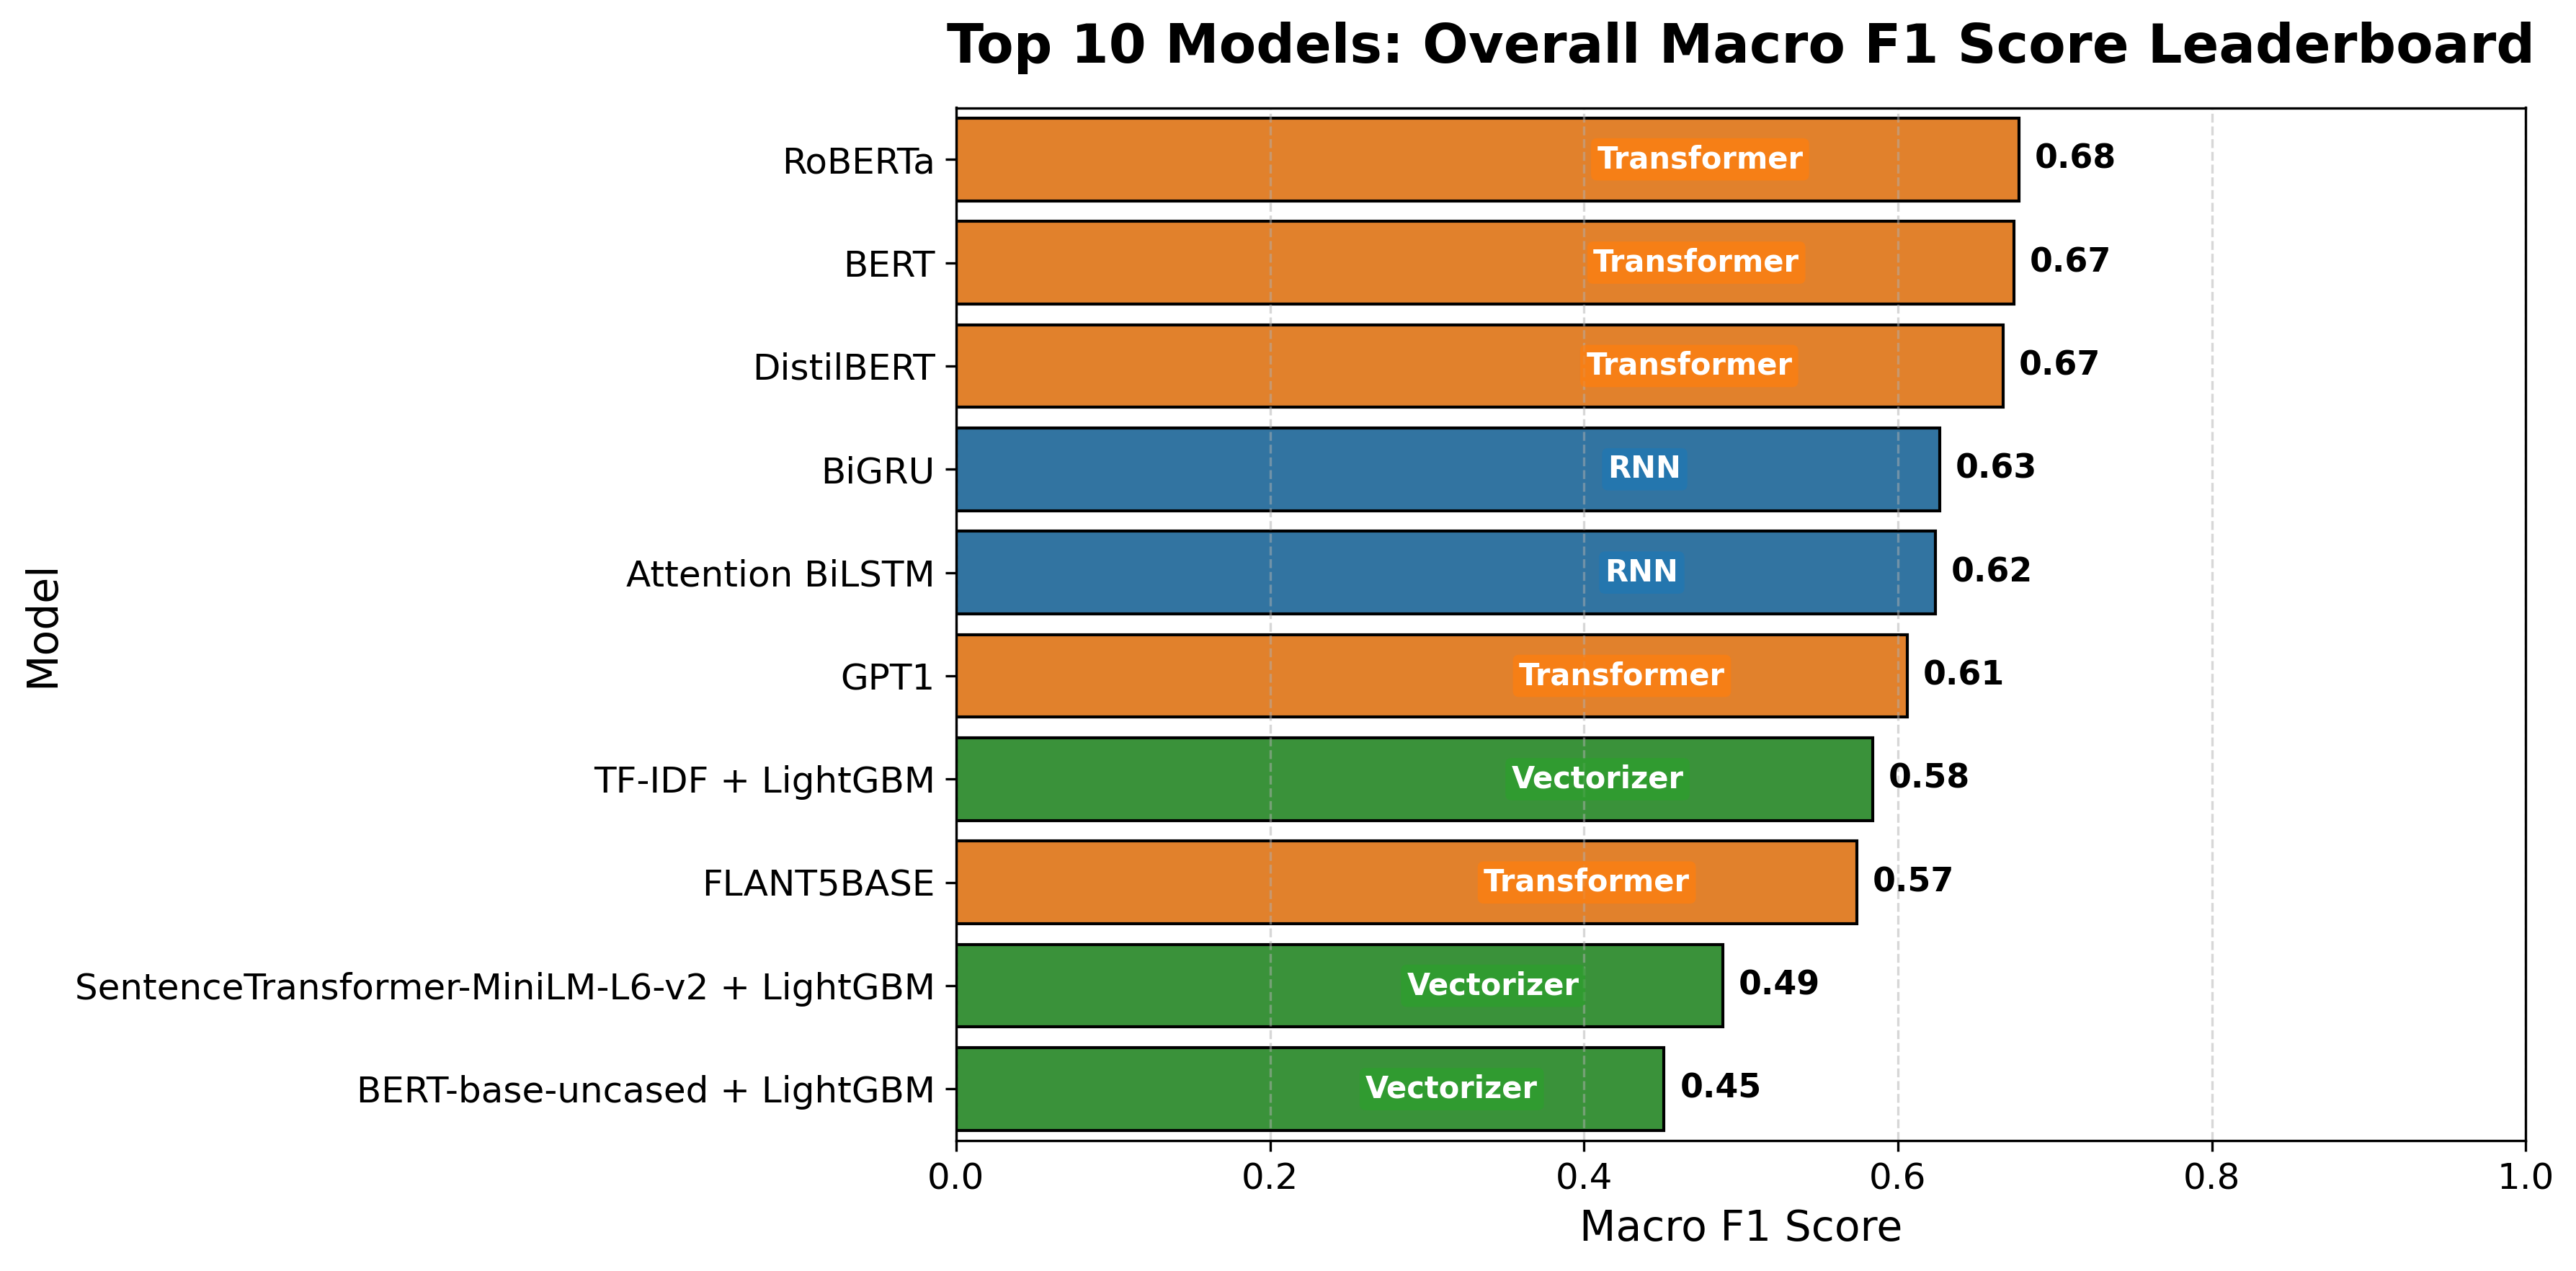
\includegraphics[width=\linewidth]{figures/macro_f1_comparison_1.png}
        \end{minipage}
        \hfill
        \begin{minipage}{0.48\linewidth}
            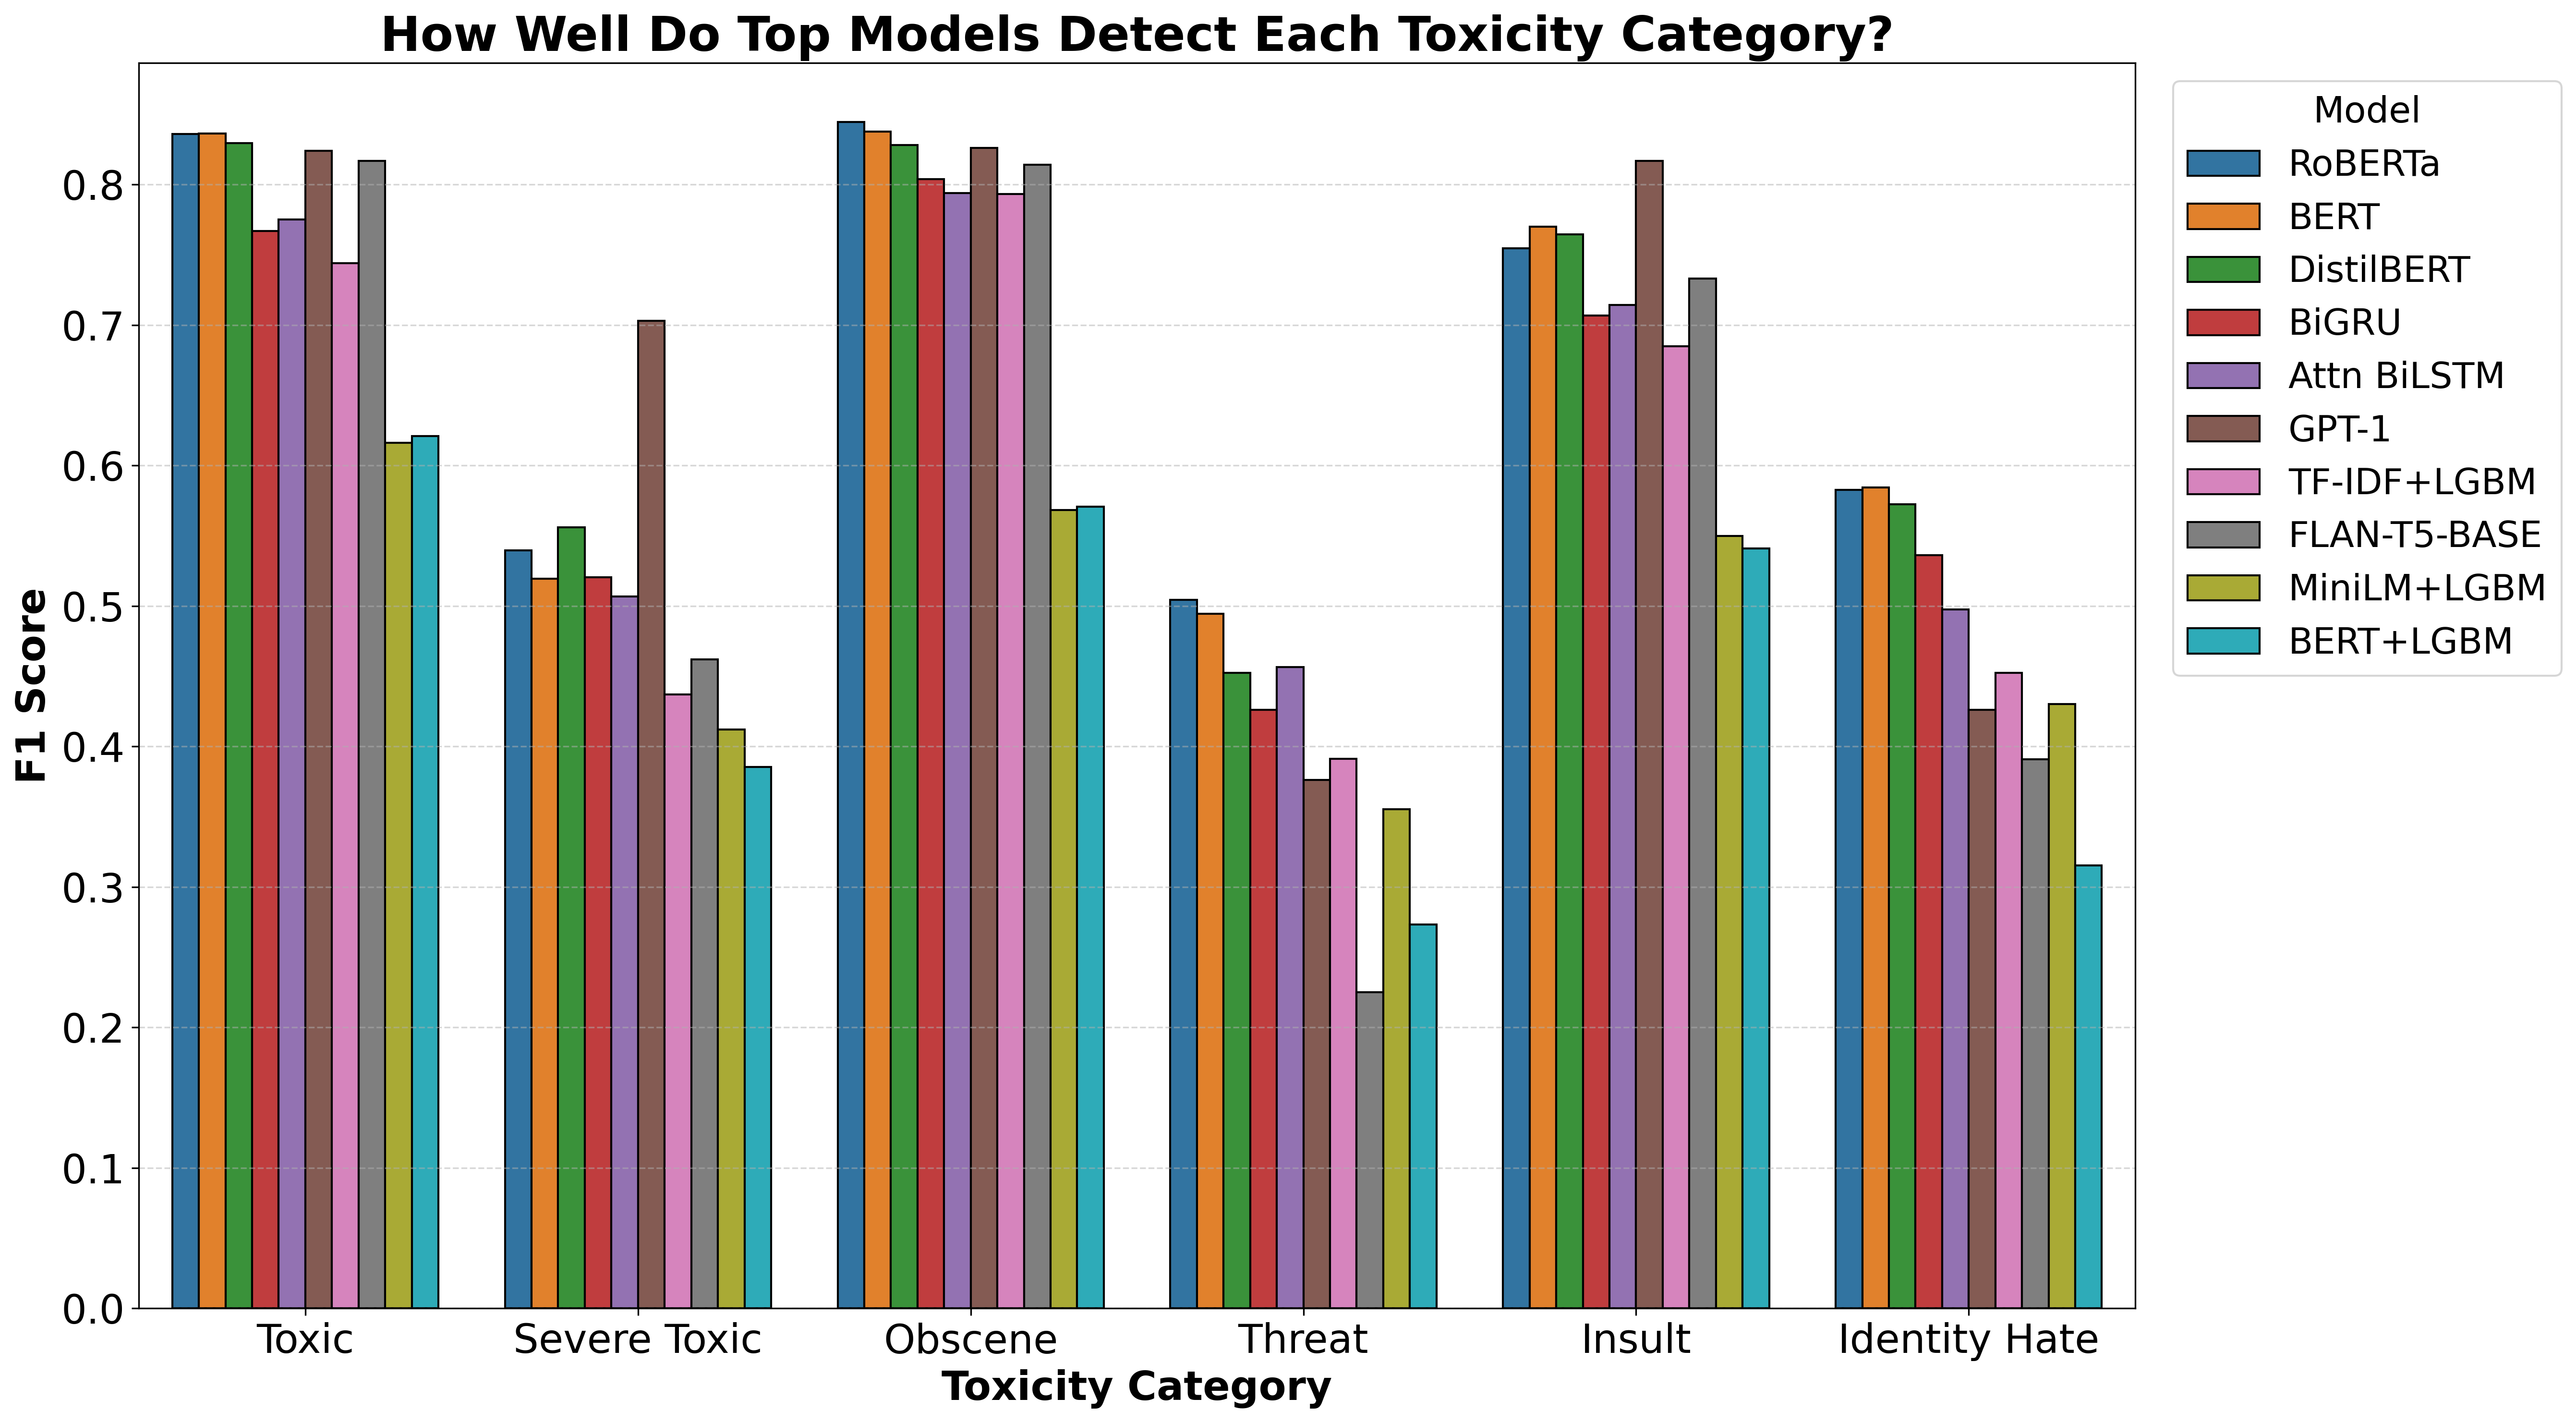
\includegraphics[width=\linewidth]{figures/per_class_f1_comparison.png}
        \end{minipage}
        \vspace{0.01em}
        \normalsize
        \begin{flushleft}
        \textbf{Summary:} Our results show that transformer models (RoBERTa, BERT, DistilBERT, GPT1) consistently outperform RNNs and vectorizer-based models both overall and across toxicity categories. However, rare classes like \textit{threat} and \textit{identity hate} remain difficult for all models. We found that even high-performing models tend to incorrectly flag neutral identity statements (e.g., ``I'm Muslim'', ``I'm gay'') as toxic, indicating bias learned from the dataset. In contrast, zero-shot large language models (LLMs) classify such statements as non-toxic, as expected. This highlights the importance of careful evaluation for unintended bias in toxic comment classifiers.
        \end{flushleft}
    \end{center}
}

